\documentclass[11pt,a4paper]{article}
\usepackage[utf8]{inputenc}
\usepackage[T1]{fontenc}
\usepackage{graphicx}
\usepackage{listings}
\usepackage{xcolor}
\usepackage{hyperref}
\usepackage{amsmath}
\usepackage{amssymb}
\usepackage{tikz}
\usepackage{geometry}
\geometry{margin=1in}

\definecolor{codegreen}{rgb}{0,0.6,0}
\definecolor{codegray}{rgb}{0.5,0.5,0.5}
\definecolor{codepurple}{rgb}{0.58,0,0.82}
\definecolor{backcolour}{rgb}{0.95,0.95,0.92}

\lstdefinestyle{pythonstyle}{
    backgroundcolor=\color{backcolour},
    commentstyle=\color{codegreen},
    keywordstyle=\color{magenta},
    numberstyle=\tiny\color{codegray},
    stringstyle=\color{codepurple},
    basicstyle=\ttfamily\small,
    breakatwhitespace=false,
    breaklines=true,
    captionpos=b,
    keepspaces=true,
    numbers=left,
    numbersep=5pt,
    showspaces=false,
    showstringspaces=false,
    showtabs=false,
    tabsize=2
}

\lstset{style=pythonstyle}

\title{Learn Compiler Design Through xDSL:\\
A Practical Course for AI/ML Engineers}
\author{Djordje Todorovic}
\date{August 2025}

\begin{document}

\maketitle

\tableofcontents
\newpage

\section{Preface: Who This Course Is For and Why Compilers Matter}

\subsection{Prerequisites and Intended Audience}

This course is designed for engineers and developers who want to understand the fundamental concepts of compiler design through hands-on experience with xDSL. To get the most out of this material, you should have:

\begin{itemize}
    \item \textbf{Python Proficiency}: Strong knowledge of Python is essential, as xDSL is a Python-native framework. You should be comfortable with classes, decorators, type hints, and the Python standard library.
    \item \textbf{Basic Programming Knowledge}: Understanding of fundamental programming concepts like functions, variables, control flow, data structures, and algorithms is required.
    \item \textbf{Machine Learning and AI Basics}: Familiarity with ML/AI concepts is crucial - you should understand tensors, neural networks, computational graphs, and optimization techniques. Experience with frameworks like PyTorch or TensorFlow will help you appreciate the compiler optimizations we'll explore.
    \item \textbf{Mathematical Foundations}: Basic understanding of linear algebra and discrete mathematics will be helpful, especially when working with optimization algorithms and graph transformations.
\end{itemize}

If you're an ML engineer curious about what happens "under the hood" when your models are compiled and optimized, or a systems programmer interested in building efficient code transformation tools, this course will bridge that gap using familiar Python syntax.

\subsection{Compilers: The Invisible Revolution That Changed Computing}

Compilers are perhaps the most transformative technology in the history of computing, yet they work so seamlessly that we rarely think about them. To understand their revolutionary impact, consider this: the Linux kernel, which powers billions of devices worldwide, was initially written in assembly language - a tedious, error-prone process where programmers had to think in terms of individual CPU instructions and memory addresses. Each line of assembly code corresponded directly to a machine instruction, making even simple tasks require hundreds of lines of code.

Then came the evolution of the C compiler. As compilers matured, they could translate high-level C code into assembly with equal or sometimes even better performance than hand-written assembly. This transformation was revolutionary - Linux could be rewritten in C, making it portable across different architectures, easier to maintain, and accessible to a broader community of developers. What once required intimate knowledge of specific CPU architectures could now be expressed in readable, maintainable code. The compiler handled the complex translation, optimization, and architecture-specific details automatically.

This same revolution continues today in machine learning. Just as C compilers freed developers from assembly, ML compilers like XLA, TVM, and MLIR free ML engineers from writing architecture-specific kernels. Your PyTorch model can run efficiently on CPUs, GPUs, TPUs, or custom accelerators, all thanks to sophisticated compiler technology working behind the scenes.

\subsection{The Core Mission: Represent and Transform}

At its heart, a compiler's job is elegantly simple yet profoundly powerful: to \textbf{represent} programs in structured forms and to \textbf{transform} these representations to achieve specific goals. Think of a compiler as a sophisticated translator that not only converts between languages but also understands the meaning of what it's translating deeply enough to improve it along the way.

This representation and transformation paradigm involves:
\begin{itemize}
    \item \textbf{Representation}: Converting source code into structured data (Abstract Syntax Trees, Intermediate Representations, Control Flow Graphs) that capture the program's semantics precisely
    \item \textbf{Analysis}: Understanding data dependencies, control flow, memory access patterns, and optimization opportunities within these representations
    \item \textbf{Transformation}: Systematically modifying these representations to optimize performance, reduce resource usage, or target specific hardware architectures
    \item \textbf{Preservation}: Ensuring that transformations maintain the original program's correctness and semantics
\end{itemize}

\subsection{The Power of Serialize, Deserialize, and Verify}

A crucial but often overlooked aspect of compiler infrastructure is the ability to serialize, deserialize, and verify intermediate representations. This capability fundamentally changes how we can work with compilers and is a cornerstone of modern compiler design.

\textbf{Why These Capabilities Matter:}
\begin{itemize}
    \item \textbf{Serialization} allows us to save the compiler's intermediate state to disk, enabling separate compilation, caching of optimization results, and distribution of compiled modules. You can pause compilation, save the IR, and resume later - or on a different machine entirely.
    \item \textbf{Deserialization} lets us load previously compiled modules, compose them together, and build large systems incrementally. This is essential for modular compilation and linking.
    \item \textbf{Verification} ensures that the IR is well-formed and obeys the type system and semantic rules. This catches errors early, enables safe transformations, and provides guarantees about program behavior. Without verification, compiler bugs could silently corrupt programs.
\end{itemize}

The xDSL infrastructure we're about to explore has these capabilities built into its core. Every operation, every transformation, and every intermediate state can be serialized to a human-readable textual format, loaded back, and verified for correctness. This isn't just a convenience feature - it's fundamental to building robust, composable compiler pipelines. You can inspect the IR at any stage, debug transformations by examining the before-and-after states, and even hand-write IR for testing.

This approach contrasts sharply with traditional compilers where the intermediate states are often opaque binary structures locked inside the compiler's memory. With xDSL (inspired by MLIR), the entire compilation pipeline becomes transparent, debuggable, and extensible. You can serialize the IR after each optimization pass, analyze what changed, and even replay specific transformations. This visibility and control make compiler development more like software engineering and less like black magic.

As you progress through this course, you'll come to appreciate how these fundamental capabilities - serialize, deserialize, and verify - enable you to build reliable, maintainable, and powerful compilation tools. They transform the compiler from a monolithic black box into a modular, inspectable, and trustworthy system.

\section{Introduction: Compilers as Representation and Transformation Engines}

\subsection{Welcome to the World of Compilers}

If you're coming from an AI/ML background, you already understand the power of transforming data through layers of abstraction. Compilers are remarkably similar: they take programs written in one representation and systematically transform them into another, more optimized or more executable form.

Think of a compiler as a sophisticated pipeline that:
\begin{enumerate}
    \item \textbf{Represents} programs as structured data (Abstract Syntax Trees, Intermediate Representations)
    \item \textbf{Transforms} these representations through a series of optimization passes
    \item \textbf{Analyzes} code to understand dependencies, patterns, and optimization opportunities
    \item \textbf{Generates} efficient target code for specific hardware
\end{enumerate}

\subsection{Why xDSL?}

xDSL is a Python-native compiler framework that makes compiler concepts accessible to Python programmers. Unlike traditional compiler frameworks written in C++ (like LLVM), xDSL allows you to:
\begin{itemize}
    \item Build compilers using familiar Python syntax
    \item Prototype and experiment quickly
    \item Understand compiler internals without low-level complexity
    \item Leverage the entire Python ecosystem for analysis and visualization
\end{itemize}

\subsection{Course Philosophy: Learn by Building}

This course takes a hands-on approach. Instead of starting with theory, we'll build small compilers and optimization passes from day one. Each concept will be introduced through practical examples that you can run, modify, and experiment with.

\subsection{What You'll Learn}

By the end of this course, you'll understand:
\begin{itemize}
    \item How compilers represent programs internally (IR - Intermediate Representations)
    \item What operations and operators mean in a compiler context
    \item How to write analysis passes that extract information from code
    \item How to implement transformations that optimize programs
    \item The connection between compiler optimizations and ML model optimization
\end{itemize}

\section{Chapter 1: Understanding Intermediate Representations (IR)}

\subsection{What is an IR?}

An Intermediate Representation (IR) is the compiler's internal language for representing programs. Just as neural networks use tensors to represent data, compilers use IRs to represent code structure and semantics.

Key properties of IRs:
\begin{itemize}
    \item \textbf{Abstract}: Higher-level than machine code, but more structured than source code
    \item \textbf{Explicit}: Makes implicit operations visible (e.g., memory allocations, type conversions)
    \item \textbf{Analyzable}: Designed for easy pattern matching and transformation
    \item \textbf{Hierarchical}: Can represent nested structures (functions, loops, blocks)
\end{itemize}

\subsection{The Compiler Pipeline: From Source to Machine Code}

Before diving into xDSL specifics, let's understand how compilers work. A compiler is traditionally divided into three main phases, each with specific responsibilities:

\subsubsection{Frontend: Understanding Your Code}

The frontend translates source code into an intermediate representation. It consists of:

\textbf{1. Lexical Analysis (Lexer/Tokenizer)}
\begin{itemize}
    \item Breaks source code into tokens (keywords, identifiers, operators)
    \item Like splitting a sentence into words
    \item Example: \texttt{"x = 42 + y"} becomes tokens: [\texttt{ID:x}, \texttt{ASSIGN}, \texttt{NUM:42}, \texttt{PLUS}, \texttt{ID:y}]
\end{itemize}

\textbf{2. Syntax Analysis (Parser)}
\begin{itemize}
    \item Builds an Abstract Syntax Tree (AST) from tokens
    \item Checks grammatical structure
    \item Like diagramming a sentence to understand its structure
\end{itemize}

\begin{lstlisting}[language=Python, caption=Simple AST Example]
# Source: x = 42 + y
# AST representation:
Assignment(
    left=Variable("x"),
    right=BinaryOp(
        op="+",
        left=Number(42),
        right=Variable("y")
    )
)
\end{lstlisting}

\textbf{3. Semantic Analysis}
\begin{itemize}
    \item Type checking: Is this operation valid?
    \item Symbol resolution: What does this variable refer to?
    \item Example: Can't add a string to a number, variables must be declared
\end{itemize}

\subsubsection{Middle-end: Optimization Central}

The middle-end works on the IR to optimize code:
\begin{itemize}
    \item \textbf{Platform-independent}: Optimizations work for any target
    \item \textbf{Examples}: Dead code elimination, constant folding, loop optimization
    \item \textbf{Multiple passes}: Each optimization is a separate pass over the IR
\end{itemize}

\subsubsection{Backend: Generating Machine Code}

The backend translates optimized IR to target-specific code:
\begin{itemize}
    \item \textbf{Instruction selection}: Choose machine instructions
    \item \textbf{Register allocation}: Assign variables to CPU registers
    \item \textbf{Instruction scheduling}: Order operations for performance
\end{itemize}

\subsection{Learning from Giants: LLVM and MLIR}

\subsubsection{LLVM: The Industry Standard}

LLVM (Low Level Virtual Machine) is the most widely used compiler infrastructure:
\begin{itemize}
    \item Powers Clang (C/C++), Swift, Rust, and many other languages
    \item Provides a well-defined IR (LLVM IR) that many frontends target
    \item Excellent tutorial: \href{https://llvm.org/docs/tutorial/MyFirstLanguageFrontend/index.html}{Kaleidoscope Tutorial}
    \item Shows how to build a complete compiler for a simple language
\end{itemize}

\begin{lstlisting}[language=C, caption=LLVM IR Example]
; LLVM IR for: int add(int a, int b) { return a + b; }
define i32 @add(i32 %a, i32 %b) {
entry:
  %sum = add i32 %a, %b
  ret i32 %sum
}
\end{lstlisting}

\subsubsection{MLIR: Multi-Level IR}

MLIR (Multi-Level Intermediate Representation) extends LLVM's concepts:
\begin{itemize}
    \item Developed by Google, now part of LLVM project
    \item Supports multiple IRs (dialects) in the same infrastructure
    \item Used by TensorFlow, PyTorch, and other ML frameworks
    \item Tutorial: \href{https://mlir.llvm.org/docs/Tutorials/Toy/}{Toy Language Tutorial}
    \item xDSL is heavily inspired by MLIR but implemented in Python
\end{itemize}

\begin{lstlisting}[caption=MLIR Example - Multiple Abstraction Levels]
// High-level ML operation
%result = "tf.MatMul"(%a, %b) : (tensor<2x3xf32>, tensor<3x4xf32>) 
                                -> tensor<2x4xf32>

// After lowering to linalg dialect
%result = linalg.matmul ins(%a, %b : memref<2x3xf32>, memref<3x4xf32>)
                       outs(%c : memref<2x4xf32>)

// After lowering to loops
scf.for %i = 0 to 2 {
  scf.for %j = 0 to 4 {
    scf.for %k = 0 to 3 {
      // actual computation
    }
  }
}
\end{lstlisting}

\subsection{Why xDSL Uses IR Instead of AST}

While traditional compilers start with AST, xDSL (like MLIR) works directly with IR because:
\begin{itemize}
    \item \textbf{Uniformity}: All transformations work on the same structure
    \item \textbf{Composability}: Easy to combine different languages/dialects
    \item \textbf{Reusability}: Optimizations work across different source languages
    \item \textbf{Analysis-friendly}: SSA form makes many analyses trivial
\end{itemize}

Think of it this way:
\begin{itemize}
    \item \textbf{AST}: Like a sentence diagram - shows structure
    \item \textbf{IR}: Like assembly with types - shows computation
\end{itemize}

\subsection{SSA Form: Single Static Assignment}

xDSL uses SSA (Single Static Assignment) form, where each variable is assigned exactly once. This is similar to functional programming and makes many analyses simpler.

\begin{lstlisting}[language=Python, caption=Traditional vs SSA Form]
# Traditional form
x = 5
x = x + 1
y = x * 2

# SSA form (conceptual)
x_0 = 5
x_1 = x_0 + 1
y_0 = x_1 * 2
\end{lstlisting}

Why SSA matters:
\begin{itemize}
    \item \textbf{No ambiguity}: Each value has exactly one definition
    \item \textbf{Easy analysis}: Use-def chains are explicit
    \item \textbf{Better optimization}: Many optimizations become simpler
    \item \textbf{Parallel-friendly}: Dependencies are clear
\end{itemize}

\subsection{Your First xDSL Program}

Let's create a simple IR program using xDSL:

\begin{lstlisting}[language=Python, caption=Creating IR in xDSL]
from xdsl.context import Context
from xdsl.dialects import builtin, arith, func
from xdsl.ir import Operation, Block, Region
from xdsl.builder import Builder

# Create a context (like a namespace for dialects)
ctx = Context()
ctx.load_dialect(builtin.Builtin)
ctx.load_dialect(arith.Arith)
ctx.load_dialect(func.Func)

# Build a simple function that adds two numbers
@Builder.implicit_region
def create_add_function():
    # Create function signature: (i32, i32) -> i32
    func_type = func.FunctionType.from_lists([builtin.i32, builtin.i32], [builtin.i32])
    
    with func.FuncOp("add", func_type, visibility="public").body:
        # Get function arguments
        arg0 = Block.current().args[0]
        arg1 = Block.current().args[1]
        
        # Create add operation
        result = arith.Addi(arg0, arg1).result
        
        # Return the result
        func.Return(result)

module = builtin.ModuleOp([create_add_function()])
print(module)
\end{lstlisting}

\subsection{Understanding IR Structure}

The IR in xDSL follows a hierarchical structure:

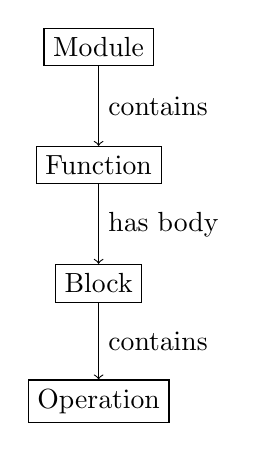
\begin{tikzpicture}[node distance=1.5cm]
    \node[draw, rectangle] (module) {Module};
    \node[draw, rectangle, below of=module] (function) {Function};
    \node[draw, rectangle, below of=function] (block) {Block};
    \node[draw, rectangle, below of=block] (operation) {Operation};
    
    \draw[->] (module) -- (function) node[midway, right] {contains};
    \draw[->] (function) -- (block) node[midway, right] {has body};
    \draw[->] (block) -- (operation) node[midway, right] {contains};
\end{tikzpicture}

\subsection{Dialects: Modular IR Design}

xDSL organizes operations into \textit{dialects} - collections of related operations and types. This is similar to how PyTorch has different modules (nn, optim, etc.).

Common dialects in xDSL:
\begin{itemize}
    \item \texttt{arith}: Arithmetic operations (add, multiply, divide)
    \item \texttt{func}: Function definitions and calls
    \item \texttt{memref}: Memory operations (like NumPy arrays)
    \item \texttt{scf}: Structured control flow (loops, conditionals)
    \item \texttt{linalg}: Linear algebra operations (matrix multiply, convolution)
\end{itemize}

\section{Chapter 2: Operations and Operators}

\subsection{What is an Operation?}

An operation in xDSL is the fundamental unit of computation. Each operation:
\begin{itemize}
    \item Has a name (e.g., \texttt{arith.addi} for integer addition)
    \item Takes input values (operands)
    \item Produces output values (results)
    \item May have attributes (compile-time constants)
    \item Can contain regions (nested blocks of operations)
\end{itemize}

\subsection{Creating Custom Operations}

Let's define a custom operation for matrix operations:

\begin{lstlisting}[language=Python, caption=Defining Custom Operations]
from xdsl.irdl import (
    IRDLOperation, 
    OpResult, 
    Operand, 
    OperandDef, 
    ResultDef,
    op_def,
    result_def
)
from xdsl.dialects.builtin import TensorType

@op_def
class MatMulOp(IRDLOperation):
    """Matrix multiplication operation"""
    name = "my_dialect.matmul"
    
    # Define operands (inputs)
    lhs = operand_def(TensorType)
    rhs = operand_def(TensorType)
    
    # Define results (outputs)
    result = result_def(TensorType)
    
    def __init__(self, lhs: Value, rhs: Value):
        super().__init__(operands=[lhs, rhs], 
                        result_types=[infer_matmul_type(lhs, rhs)])
    
    def verify(self):
        """Verify that the operation is well-formed"""
        # Check that dimensions are compatible
        lhs_shape = self.lhs.type.shape
        rhs_shape = self.rhs.type.shape
        
        if lhs_shape[-1] != rhs_shape[0]:
            raise ValueError("Incompatible matrix dimensions")
\end{lstlisting}

\subsection{Operation Semantics}

Every operation has well-defined semantics - what it means to execute that operation:

\begin{lstlisting}[language=Python, caption=Operation Semantics Example]
# Arithmetic operations
add_op = arith.Addi(a, b)  # result = a + b
mul_op = arith.Muli(a, b)  # result = a * b

# Memory operations  
alloc_op = memref.Alloc.get(shape=[10, 20], element_type=f32)  # Allocate 10x20 array
load_op = memref.Load.get(memref_value, indices)  # Load from memory
store_op = memref.Store.get(value, memref_value, indices)  # Store to memory

# Control flow operations
for_op = scf.For(lower_bound, upper_bound, step) # for loop
if_op = scf.If(condition, has_else=True)  # if-then-else
\end{lstlisting}

\subsection{Attributes vs Operands}

Understanding the difference between attributes and operands is crucial:

\begin{itemize}
    \item \textbf{Attributes}: Compile-time constants (shapes, types, flags)
    \item \textbf{Operands}: Runtime values (variables, intermediate results)
\end{itemize}

\begin{lstlisting}[language=Python, caption=Attributes vs Operands]
# Constant has an attribute (the value)
const = arith.Constant.from_int_and_width(42, 32)  # 42 is an attribute

# Add has operands (runtime values)
result = arith.Addi(x, y)  # x and y are operands

# Alloc has attributes (shape) but no operands
mem = memref.Alloc.get(shape=[100], element_type=f32)  # shape is attribute
\end{lstlisting}

\section{Chapter 3: Analysis Passes}

\subsection{What is Analysis?}

Analysis passes extract information from IR without modifying it. They answer questions like:
\begin{itemize}
    \item Which variables are used where? (Use-Def Analysis)
    \item Which operations can run in parallel? (Dependency Analysis)
    \item What are the loop bounds? (Range Analysis)
    \item Which operations are dead code? (Liveness Analysis)
\end{itemize}

\subsection{Writing a Simple Analysis Pass}

Let's write an analysis that counts operations by type:

\begin{lstlisting}[language=Python, caption=Operation Counter Analysis]
from xdsl.passes import Pass
from xdsl.ir import Operation, OpResult
from collections import defaultdict

class OperationCounterPass(Pass):
    """Count operations by type in the IR"""
    
    name = "count-ops"
    
    def apply(self, module: builtin.ModuleOp) -> None:
        op_counts = defaultdict(int)
        
        # Walk through all operations in the module
        for op in module.walk():
            op_counts[op.name] += 1
        
        # Print analysis results
        print("Operation counts:")
        for op_name, count in sorted(op_counts.items()):
            print(f"  {op_name}: {count}")
        
        # Store results for use by other passes
        self.op_counts = op_counts
\end{lstlisting}

\subsection{Use-Def Chains}

Use-Def chains track where values are defined and used:

\begin{lstlisting}[language=Python, caption=Use-Def Analysis]
class UseDefAnalysis(Pass):
    """Analyze use-def relationships"""
    
    def apply(self, module: builtin.ModuleOp) -> None:
        # Build use-def chains
        for op in module.walk():
            for result in op.results:
                print(f"Value {result} defined by {op.name}")
                print(f"  Used by: {[use.operation.name for use in result.uses]}")
    
    def find_unused_values(self, module: builtin.ModuleOp) -> list[OpResult]:
        """Find values that are never used"""
        unused = []
        for op in module.walk():
            for result in op.results:
                if not result.uses:
                    unused.append(result)
        return unused
\end{lstlisting}

\subsection{Dominance Analysis}

Dominance tells us which operations must execute before others:

\begin{lstlisting}[language=Python, caption=Dominance Analysis]
from xdsl.ir import Block
from xdsl.irdl.dominance import DominanceInfo

class DominanceAnalysis(Pass):
    """Analyze control flow dominance"""
    
    def apply(self, module: builtin.ModuleOp) -> None:
        # For each function in the module
        for func_op in module.body.ops:
            if isinstance(func_op, func.FuncOp):
                dom_info = DominanceInfo(func_op.body)
                
                # Check dominance relationships
                for block in func_op.body.blocks:
                    dominators = dom_info.get_dominators(block)
                    print(f"Block {block} dominated by: {dominators}")
\end{lstlisting}

\subsection{Dataflow Analysis}

Dataflow analysis propagates information through the program:

\begin{lstlisting}[language=Python, caption=Constant Propagation Analysis]
class ConstantPropagationAnalysis(Pass):
    """Analyze which values are compile-time constants"""
    
    def apply(self, module: builtin.ModuleOp) -> None:
        known_constants = {}
        
        # First pass: identify constants
        for op in module.walk():
            if isinstance(op, arith.Constant):
                known_constants[op.result] = op.value.value
        
        # Iteratively propagate constants
        changed = True
        while changed:
            changed = False
            for op in module.walk():
                if isinstance(op, arith.Addi):
                    # If both operands are known constants
                    if (op.lhs in known_constants and 
                        op.rhs in known_constants):
                        result_value = (known_constants[op.lhs] + 
                                      known_constants[op.rhs])
                        if op.result not in known_constants:
                            known_constants[op.result] = result_value
                            changed = True
        
        return known_constants
\end{lstlisting}

\section{Chapter 4: Transformations and Optimizations}

\subsection{What is a Transformation?}

Transformations modify the IR to improve performance, reduce code size, or prepare for further optimizations. Unlike analysis passes, transformations actually change the program structure.

Key principles:
\begin{itemize}
    \item \textbf{Correctness}: Must preserve program semantics
    \item \textbf{Profitability}: Should improve some metric (speed, size, power)
    \item \textbf{Composability}: Should work well with other transformations
\end{itemize}

\subsection{Pattern-Based Rewriting}

xDSL provides powerful pattern matching for transformations:

\begin{lstlisting}[language=Python, caption=Simple Algebraic Optimization]
from xdsl.pattern_rewriter import (
    PatternRewriter, 
    RewritePattern,
    op_type_rewrite_pattern
)

class FoldAddZero(RewritePattern):
    """Fold x + 0 -> x"""
    
    @op_type_rewrite_pattern
    def match_and_rewrite(self, op: arith.Addi, 
                         rewriter: PatternRewriter) -> None:
        # Check if right operand is zero
        if isinstance(op.rhs.owner, arith.Constant):
            if op.rhs.owner.value.value == 0:
                # Replace all uses of the add with the left operand
                rewriter.replace_op(op, [op.lhs])
                return
        
        # Check if left operand is zero  
        if isinstance(op.lhs.owner, arith.Constant):
            if op.lhs.owner.value.value == 0:
                rewriter.replace_op(op, [op.rhs])
\end{lstlisting}

\subsection{Common Optimizations}

\subsubsection{Dead Code Elimination}

Remove operations whose results are never used:

\begin{lstlisting}[language=Python, caption=Dead Code Elimination]
class DeadCodeElimination(Pass):
    """Remove unused operations"""
    
    def apply(self, module: builtin.ModuleOp) -> None:
        ops_to_remove = []
        
        for op in module.walk():
            # Skip operations with side effects
            if self.has_side_effects(op):
                continue
                
            # Check if any results are used
            all_dead = all(not result.uses for result in op.results)
            
            if all_dead:
                ops_to_remove.append(op)
        
        # Remove dead operations
        for op in ops_to_remove:
            op.erase()
    
    def has_side_effects(self, op: Operation) -> bool:
        """Check if operation has side effects"""
        # Memory writes, function calls, etc.
        return isinstance(op, (memref.Store, func.Call))
\end{lstlisting}

\subsubsection{Common Subexpression Elimination}

Identify and eliminate redundant computations:

\begin{lstlisting}[language=Python, caption=Common Subexpression Elimination]
class CommonSubexpressionElimination(Pass):
    """Eliminate redundant computations"""
    
    def apply(self, module: builtin.ModuleOp) -> None:
        # Map from (op_type, operands) to result
        expression_map = {}
        
        for op in module.walk():
            if self.is_pure(op):
                # Create a key for this expression
                key = self.get_expression_key(op)
                
                if key in expression_map:
                    # Found duplicate - replace with existing
                    existing_result = expression_map[key]
                    op.results[0].replace_by(existing_result)
                    op.erase()
                else:
                    # First occurrence - remember it
                    expression_map[key] = op.results[0]
    
    def get_expression_key(self, op: Operation):
        """Create hashable key for expression"""
        return (op.name, tuple(op.operands))
\end{lstlisting}

\subsubsection{Loop Optimizations}

Optimize loop structures for better performance:

\begin{lstlisting}[language=Python, caption=Loop Unrolling]
class LoopUnrolling(Pass):
    """Unroll small loops"""
    
    def apply(self, module: builtin.ModuleOp) -> None:
        for op in module.walk():
            if isinstance(op, scf.For):
                if self.should_unroll(op):
                    self.unroll_loop(op)
    
    def should_unroll(self, loop: scf.For) -> bool:
        """Decide if loop should be unrolled"""
        # Get loop bounds if constant
        if (isinstance(loop.lb.owner, arith.Constant) and
            isinstance(loop.ub.owner, arith.Constant)):
            lb = loop.lb.owner.value.value
            ub = loop.ub.owner.value.value
            iterations = ub - lb
            
            # Unroll small loops
            return iterations <= 4
        return False
    
    def unroll_loop(self, loop: scf.For):
        """Completely unroll a loop"""
        # Clone loop body for each iteration
        # Update induction variable references
        # Remove original loop
        pass  # Implementation details omitted
\end{lstlisting}

\subsection{Lowering Transformations}

Lowering transforms high-level operations into simpler ones:

\begin{lstlisting}[language=Python, caption=Lowering High-Level Operations]
class LowerMatrixOps(Pass):
    """Lower matrix operations to loops"""
    
    def apply(self, module: builtin.ModuleOp) -> None:
        for op in module.walk():
            if isinstance(op, MatMulOp):
                self.lower_matmul(op)
    
    def lower_matmul(self, matmul: MatMulOp):
        """Lower matmul to three nested loops"""
        builder = Builder.before(matmul)
        
        # Get dimensions
        m, k = matmul.lhs.type.shape
        _, n = matmul.rhs.type.shape
        
        # Allocate result
        result = builder.insert(memref.Alloc.get([m, n], f32))
        
        # Generate three nested loops
        with builder.insert(scf.For(0, m, 1)) as i:
            with builder.insert(scf.For(0, n, 1)) as j:
                # Initialize accumulator
                zero = builder.insert(arith.Constant.from_float(0.0, f32))
                
                with builder.insert(scf.For(0, k, 1, [zero])) as (k_idx, acc):
                    # Load elements
                    a_elem = builder.insert(memref.Load(matmul.lhs, [i, k_idx]))
                    b_elem = builder.insert(memref.Load(matmul.rhs, [k_idx, j]))
                    
                    # Multiply and accumulate
                    prod = builder.insert(arith.Mulf(a_elem, b_elem))
                    new_acc = builder.insert(arith.Addf(acc, prod))
                    
                    scf.Yield(new_acc)
                
                # Store result
                builder.insert(memref.Store(acc, result, [i, j]))
        
        # Replace matmul with lowered result
        matmul.results[0].replace_by(result)
        matmul.erase()
\end{lstlisting}

\section{Chapter 5: Practical Examples}

\subsection{Building a Simple Expression Compiler}

Let's build a complete compiler for arithmetic expressions:

\begin{lstlisting}[language=Python, caption=Expression Compiler]
from dataclasses import dataclass
from typing import Union

# Define AST nodes
@dataclass
class Expr:
    pass

@dataclass
class Number(Expr):
    value: int

@dataclass  
class BinaryOp(Expr):
    left: Expr
    op: str
    right: Expr

# Parser (simplified)
def parse(text: str) -> Expr:
    """Parse expression like '2 + 3 * 4'"""
    # Implementation omitted for brevity
    pass

# IR Generator
class ExprIRGen:
    def __init__(self):
        self.builder = Builder()
        
    def compile(self, expr: Expr) -> OpResult:
        """Compile expression to xDSL IR"""
        if isinstance(expr, Number):
            return arith.Constant.from_int_and_width(
                expr.value, 32).result
        
        elif isinstance(expr, BinaryOp):
            left = self.compile(expr.left)
            right = self.compile(expr.right)
            
            if expr.op == '+':
                return arith.Addi(left, right).result
            elif expr.op == '*':
                return arith.Muli(left, right).result
            # ... other operations

# Optimizer
def optimize(module: builtin.ModuleOp):
    """Apply optimization passes"""
    passes = [
        ConstantFolding(),
        CommonSubexpressionElimination(),
        DeadCodeElimination(),
    ]
    
    for pass_instance in passes:
        pass_instance.apply(module)

# Complete pipeline
def compile_expression(text: str):
    # Parse
    ast = parse(text)
    
    # Generate IR
    ir_gen = ExprIRGen()
    result = ir_gen.compile(ast)
    
    # Wrap in module
    module = builtin.ModuleOp([
        func.FuncOp("compute", 
                   func.FunctionType.from_lists([], [builtin.i32]),
                   body=[func.Return(result)])
    ])
    
    # Optimize
    optimize(module)
    
    return module
\end{lstlisting}

\subsection{Implementing a Domain-Specific Optimization}

Let's create an optimization for neural network operations:

\begin{lstlisting}[language=Python, caption=Neural Network Optimization]
class FuseBatchNormIntoConv(Pass):
    """Fuse batch normalization into preceding convolution"""
    
    def apply(self, module: builtin.ModuleOp) -> None:
        for conv in module.walk():
            if isinstance(conv, nn.Conv2d):
                # Look for batch norm following conv
                for use in conv.result.uses:
                    if isinstance(use.operation, nn.BatchNorm2d):
                        self.fuse(conv, use.operation)
    
    def fuse(self, conv: nn.Conv2d, bn: nn.BatchNorm2d):
        """Fuse batch norm parameters into convolution"""
        # Extract batch norm parameters
        gamma = bn.gamma  # scale
        beta = bn.beta    # shift
        mean = bn.running_mean
        var = bn.running_var
        eps = bn.eps
        
        # Compute fused weights and bias
        std = sqrt(var + eps)
        fused_weight = conv.weight * (gamma / std)
        fused_bias = gamma * (conv.bias - mean) / std + beta
        
        # Create new convolution with fused parameters
        fused_conv = nn.Conv2d(
            weight=fused_weight,
            bias=fused_bias,
            # ... other conv parameters
        )
        
        # Replace conv -> bn with fused conv
        bn.result.replace_by(fused_conv.result)
        conv.erase()
        bn.erase()
\end{lstlisting}

\subsection{Building a Mini ML Compiler}

Let's create a compiler for a subset of ML operations:

\begin{lstlisting}[language=Python, caption=Mini ML Compiler]
# Define ML dialect
@dialect_def
class MLDialect(Dialect):
    name = "ml"

@op_def
class LinearOp(IRDLOperation):
    """Linear layer: y = Wx + b"""
    name = "ml.linear"
    
    input = operand_def(TensorType)
    weight = operand_def(TensorType)  
    bias = operand_def(TensorType)
    
    output = result_def(TensorType)

@op_def
class ReluOp(IRDLOperation):
    """ReLU activation"""
    name = "ml.relu"
    
    input = operand_def(TensorType)
    output = result_def(TensorType)

# Optimization: Fuse Linear + ReLU
class FuseLinearRelu(RewritePattern):
    @op_type_rewrite_pattern
    def match_and_rewrite(self, relu: ReluOp, 
                         rewriter: PatternRewriter):
        # Check if input is from linear
        if isinstance(relu.input.owner, LinearOp):
            linear = relu.input.owner
            
            # Create fused operation
            fused = LinearReluOp(
                linear.input, 
                linear.weight,
                linear.bias
            )
            
            # Replace both ops with fused version
            rewriter.replace_op(relu, [fused.output])
            rewriter.erase_op(linear)

# Lower to hardware operations
class LowerMLToHardware(Pass):
    """Lower ML ops to target hardware"""
    
    def apply(self, module: builtin.ModuleOp):
        target = self.get_target()  # CPU, GPU, TPU, etc.
        
        for op in module.walk():
            if isinstance(op, LinearOp):
                if target == "gpu":
                    self.lower_linear_to_cublas(op)
                elif target == "cpu":
                    self.lower_linear_to_loops(op)
\end{lstlisting}

\section{Chapter 6: Advanced Topics}

\subsection{Multi-Level IR and Progressive Lowering}

Real compilers use multiple levels of abstraction:

\begin{lstlisting}[language=Python, caption=Multi-Level Compilation Pipeline]
class CompilationPipeline:
    """Progressive lowering through multiple IR levels"""
    
    def compile(self, source_code: str) -> str:
        # Level 1: High-level ML operations
        ml_ir = parse_to_ml_dialect(source_code)
        ml_ir = optimize_ml_level(ml_ir)
        
        # Level 2: Linear algebra operations
        linalg_ir = lower_ml_to_linalg(ml_ir)
        linalg_ir = optimize_linalg_level(linalg_ir)
        
        # Level 3: Loops and memory operations
        loop_ir = lower_linalg_to_loops(linalg_ir)
        loop_ir = optimize_loops(loop_ir)
        
        # Level 4: Target-specific operations
        target_ir = lower_to_target(loop_ir)
        target_ir = optimize_target_specific(target_ir)
        
        # Code generation
        return generate_code(target_ir)
\end{lstlisting}

\subsection{Cost Models and Autotuning}

Choosing the best optimization requires understanding costs:

\begin{lstlisting}[language=Python, caption=Cost-Based Optimization]
class CostModel:
    """Estimate operation costs"""
    
    def estimate_cost(self, op: Operation) -> float:
        if isinstance(op, arith.Mulf):
            return 1.0  # FP multiply cost
        elif isinstance(op, memref.Load):
            return self.memory_latency(op)
        elif isinstance(op, scf.For):
            iterations = self.analyze_trip_count(op)
            body_cost = sum(self.estimate_cost(body_op) 
                          for body_op in op.body.walk())
            return iterations * body_cost

class AutotuningPass(Pass):
    """Try different optimization strategies"""
    
    def apply(self, module: builtin.ModuleOp):
        strategies = [
            self.try_vectorization,
            self.try_loop_tiling,
            self.try_parallelization,
        ]
        
        best_module = module
        best_cost = self.cost_model.estimate_cost(module)
        
        for strategy in strategies:
            candidate = strategy(module.clone())
            cost = self.cost_model.estimate_cost(candidate)
            
            if cost < best_cost:
                best_module = candidate
                best_cost = cost
        
        return best_module
\end{lstlisting}

\subsection{Connection to ML Compilation}

Modern ML frameworks are essentially compilers:

\begin{itemize}
    \item \textbf{PyTorch JIT}: Traces Python code to TorchScript IR
    \item \textbf{TensorFlow XLA}: Compiles TF graphs to optimized kernels
    \item \textbf{JAX}: Uses XLA for JIT compilation
    \item \textbf{Apache TVM}: Optimizes ML models for various hardware
\end{itemize}

The concepts you've learned apply directly:
\begin{itemize}
    \item \textbf{Graph optimization} = IR transformation
    \item \textbf{Kernel fusion} = Operation merging
    \item \textbf{Memory planning} = Register allocation
    \item \textbf{Quantization} = Type lowering
\end{itemize}

\section{Chapter 7: Hands-On Exercises}

\subsection{Introduction: Learning by Doing}

The exercises in this chapter are designed to solidify your understanding of compiler concepts through practical implementation. Each exercise builds upon the concepts we've covered, challenging you to apply your knowledge in increasingly sophisticated ways. These aren't just academic exercises - they mirror real-world compiler engineering challenges you'll encounter in production systems.

\textbf{Goals of These Exercises:}
\begin{itemize}
    \item \textbf{Reinforce Core Concepts}: Apply IR manipulation, pattern matching, and transformation techniques in practice
    \item \textbf{Develop Compiler Intuition}: Understand trade-offs between different optimization strategies
    \item \textbf{Build Debugging Skills}: Learn to verify correctness and debug transformation passes
    \item \textbf{Connect Theory to Practice}: See how abstract concepts translate to real optimizations
\end{itemize}

\subsection{Exercise 1: Build Your Own Optimizer - Store-Load Forwarding}

\subsubsection{Context and Motivation}

Memory operations are often bottlenecks in program performance. When a program stores a value to memory and immediately loads it back, we're wasting cycles on unnecessary memory traffic. Store-load forwarding is a crucial optimization in modern compilers and CPUs that eliminates these redundant operations.

\textbf{Real-World Impact:} This optimization is so important that modern CPUs implement it in hardware. By doing it in the compiler, we can eliminate the operations entirely, reducing both memory bandwidth and instruction count.

\textbf{What You'll Learn:}
\begin{itemize}
    \item How to track data flow through memory operations
    \item Alias analysis basics (when is it safe to forward?)
    \item The importance of maintaining program correctness during optimization
    \item How to reason about memory dependencies
\end{itemize}

\begin{lstlisting}[language=Python, caption=Exercise: Store-Load Forwarding]
class StoreLoadForwarding(Pass):
    """Forward stored values to subsequent loads
    
    Transform patterns like:
        memref.store %value, %mem[%i, %j]
        %loaded = memref.load %mem[%i, %j]
    Into:
        memref.store %value, %mem[%i, %j]
        // Use %value directly instead of %loaded
    """
    
    def apply(self, module: builtin.ModuleOp):
        # TODO: Your implementation here
        # Step 1: Build a map of recent stores for each memory location
        # Step 2: For each load, check if we have a recent store
        # Step 3: Verify indices match exactly (be conservative!)
        # Step 4: Check for intervening operations that might invalidate
        # Step 5: Replace load result with stored value
        
        # Hints:
        # - Start simple: handle only same-block forwarding
        # - Be conservative: only forward when indices are identical
        # - Watch for: function calls, other stores to same array
        # - Remember: correctness > performance
        pass

    def can_forward(self, store_op, load_op):
        """Check if it's safe to forward from store to load"""
        # TODO: Implement safety checks
        pass
\end{lstlisting}

\subsubsection{Testing Your Implementation}

\begin{lstlisting}[language=Python, caption=Test Cases for Store-Load Forwarding]
def test_store_load_forwarding():
    """Test your optimization works correctly"""
    
    # Test case 1: Simple forwarding
    # store 42 to mem[0]
    # load from mem[0]  <-- should be replaced with 42
    
    # Test case 2: Different indices (no forwarding)
    # store 42 to mem[0]
    # load from mem[1]  <-- should NOT be forwarded
    
    # Test case 3: Intervening store
    # store 42 to mem[0]
    # store 100 to mem[0]
    # load from mem[0]  <-- should get 100, not 42
    
    # Test case 4: Across basic blocks (advanced)
    # Requires dominance analysis
\end{lstlisting}

\subsection{Exercise 2: Create a Custom Dialect - Quantum Computing}

\subsubsection{Context and Motivation}

Quantum computing represents a fundamentally different computational model. By creating a quantum dialect, you'll learn how compiler infrastructure can be extended to support entirely new paradigms. This exercise demonstrates xDSL's extensibility and teaches you to think about computation abstractly.

\textbf{Why This Matters:} As new computational paradigms emerge (quantum, neuromorphic, photonic), the ability to quickly prototype new compiler infrastructure becomes crucial. This exercise teaches you the skills needed to support future computing platforms.

\textbf{What You'll Learn:}
\begin{itemize}
    \item How to design operations for non-standard computation models
    \item Type system design for domain-specific constraints
    \item Verification of domain-specific invariants
    \item Lowering from high-level domain concepts to implementation
\end{itemize}

\begin{lstlisting}[language=Python, caption=Exercise: Quantum Dialect]
from xdsl.irdl import irdl_op_definition, irdl_attr_definition
from xdsl.ir import OpResult, SSAValue

@dialect_def
class QuantumDialect(Dialect):
    name = "quantum"

# TODO: Define quantum-specific types
@irdl_attr_definition
class QubitType(TypeAttribute):
    """Type representing a quantum bit"""
    name = "quantum.qubit"

@irdl_attr_definition  
class QuantumRegisterType(TypeAttribute):
    """Type for quantum register of n qubits"""
    name = "quantum.qreg"
    size: int

# TODO: Define quantum gates
@irdl_op_definition
class HadamardOp(IRDLOperation):
    """Hadamard gate: creates superposition"""
    name = "quantum.h"
    
    input_qubit = operand_def(QubitType)
    output_qubit = result_def(QubitType)
    
    def verify(self):
        """Verify operation is well-formed"""
        # Hadamard is always valid on a single qubit
        pass

@irdl_op_definition
class CNOTOp(IRDLOperation):
    """Controlled-NOT gate"""
    name = "quantum.cnot"
    
    control = operand_def(QubitType)
    target = operand_def(QubitType)
    
    # CNOT modifies both qubits
    new_control = result_def(QubitType)
    new_target = result_def(QubitType)

@irdl_op_definition
class MeasureOp(IRDLOperation):
    """Measure qubit, collapsing to classical bit"""
    name = "quantum.measure"
    
    qubit = operand_def(QubitType)
    classical_bit = result_def(IntegerType(1))

# TODO: Optimization passes
class QuantumCircuitOptimizer(Pass):
    """Optimize quantum circuits"""
    
    def apply(self, module: builtin.ModuleOp):
        # TODO: Implement optimizations like:
        # - Gate cancellation (H·H = I)
        # - Gate commutation 
        # - Circuit depth reduction
        pass
\end{lstlisting}

\subsubsection{Challenge Extensions}
\begin{itemize}
    \item Implement quantum circuit simulation
    \item Add error correction operations
    \item Create a cost model for quantum operations
    \item Implement decomposition to basic gate sets
\end{itemize}

\subsection{Exercise 3: Implement Vectorization}

\subsubsection{Context and Motivation}

Modern processors have SIMD (Single Instruction, Multiple Data) units that can process multiple data elements simultaneously. Vectorization transforms scalar operations to leverage these capabilities, often providing 4-8x speedups. This is a cornerstone optimization in high-performance computing.

\textbf{Industry Relevance:} Every production compiler implements auto-vectorization. ML frameworks rely heavily on vectorized operations for performance. Understanding vectorization is essential for performance engineering.

\textbf{What You'll Learn:}
\begin{itemize}
    \item How to identify vectorizable patterns
    \item Dependency analysis for parallel execution
    \item Handling edge cases (loop remainders, alignment)
    \item Cost modeling for vectorization decisions
\end{itemize}

\begin{lstlisting}[language=Python, caption=Exercise: Auto-Vectorization]
class Vectorization(Pass):
    """Automatically vectorize loops
    
    Transform:
        for i in range(n):
            c[i] = a[i] + b[i]
    
    Into:
        for i in range(0, n-4, 4):
            c[i:i+4] = a[i:i+4] + b[i:i+4]  # Vector operation
        for i in range(n-n%4, n):
            c[i] = a[i] + b[i]  # Scalar remainder
    """
    
    def __init__(self, vector_width=4):
        self.vector_width = vector_width
    
    def apply(self, module: builtin.ModuleOp):
        for loop in self.find_loops(module):
            if self.is_vectorizable(loop):
                self.vectorize_loop(loop)
    
    def is_vectorizable(self, loop: scf.For) -> bool:
        """Check if loop can be vectorized"""
        # TODO: Check for:
        # 1. No loop-carried dependencies
        # 2. Contiguous memory access
        # 3. Supported operations (add, mul, etc.)
        # 4. No control flow in loop body
        pass
    
    def vectorize_loop(self, loop: scf.For):
        """Transform loop to use vector operations"""
        # TODO: Implementation steps:
        # 1. Create vector loop with stride = vector_width
        # 2. Replace scalar ops with vector ops
        # 3. Create remainder loop for n % vector_width iterations
        # 4. Update memory operations to vector loads/stores
        pass
    
    def analyze_dependencies(self, loop: scf.For) -> bool:
        """Check for loop-carried dependencies"""
        # TODO: Implement dependency analysis
        # Look for patterns like a[i] = a[i-1] + b[i]
        pass
\end{lstlisting}

\subsubsection{Advanced Challenges}
\begin{itemize}
    \item Handle non-unit stride access patterns
    \item Implement cost model to decide when vectorization is profitable
    \item Support reduction operations (sum, max)
    \item Handle conditional operations with masking
\end{itemize}

\subsection{Exercise 4: Build a Simple JIT Compiler}

\subsubsection{Context and Motivation}

Just-In-Time compilation bridges the gap between interpretation and ahead-of-time compilation. By compiling code at runtime, JIT compilers can optimize based on actual execution patterns. This exercise gives you hands-on experience with the full compilation pipeline.

\textbf{Real-World Applications:} JIT compilation powers JavaScript engines (V8), Java VMs (HotSpot), Python (PyPy), and ML frameworks (JAX, PyTorch). Understanding JIT compilation is crucial for modern system design.

\textbf{What You'll Learn:}
\begin{itemize}
    \item The complete compilation pipeline from source to execution
    \item Runtime code generation techniques
    \item Optimization decisions based on runtime information
    \item Integration between compiled and interpreted code
\end{itemize}

\begin{lstlisting}[language=Python, caption=Exercise: JIT Compiler]
import ctypes
from typing import Dict, Callable

class ExpressionJIT:
    """JIT compile and execute mathematical expressions
    
    This JIT compiler will:
    1. Parse expressions into AST
    2. Generate xDSL IR
    3. Optimize the IR
    4. Generate executable code
    5. Return a callable Python function
    """
    
    def __init__(self):
        self.cache: Dict[str, Callable] = {}
        self.optimization_level = 2
    
    def compile(self, expr_string: str) -> Callable:
        """Compile expression to native function"""
        
        # Check cache first
        if expr_string in self.cache:
            return self.cache[expr_string]
        
        # Step 1: Parse expression
        ast = self.parse_expression(expr_string)
        
        # Step 2: Generate IR
        ir_module = self.generate_ir(ast)
        
        # Step 3: Optimize
        if self.optimization_level > 0:
            ir_module = self.optimize_ir(ir_module)
        
        # Step 4: Generate machine code
        machine_code = self.generate_code(ir_module)
        
        # Step 5: Create callable wrapper
        func = self.create_callable(machine_code)
        
        # Cache for future use
        self.cache[expr_string] = func
        
        return func
    
    def parse_expression(self, expr: str):
        """Parse expression into AST"""
        # TODO: Implement expression parser
        # Support: numbers, variables, +, -, *, /, parentheses
        # Example: "x * 2 + y" -> BinaryOp('+', BinaryOp('*', Var('x'), Num(2)), Var('y'))
        pass
    
    def generate_ir(self, ast) -> builtin.ModuleOp:
        """Generate xDSL IR from AST"""
        # TODO: Create IR module with function
        # Function should take dict of variables, return result
        pass
    
    def optimize_ir(self, module: builtin.ModuleOp) -> builtin.ModuleOp:
        """Apply optimization passes"""
        passes = [
            ConstantFolding(),
            CommonSubexpressionElimination(),
            DeadCodeElimination(),
        ]
        
        for opt_pass in passes:
            opt_pass.apply(module)
        
        return module
    
    def generate_code(self, module: builtin.ModuleOp) -> bytes:
        """Generate machine code or Python bytecode"""
        # TODO: Options:
        # 1. Generate Python bytecode using 'compile()'
        # 2. Use LLVM bindings to generate native code
        # 3. Generate C code and compile with ctypes
        pass
    
    def create_callable(self, code: bytes) -> Callable:
        """Create Python-callable function from machine code"""
        # TODO: Wrap machine code in Python-callable interface
        pass

# Usage example:
jit = ExpressionJIT()
f = jit.compile("x * 2 + y")
result = f(x=5, y=3)  # Should return 13

# Advanced: Support for conditionals
g = jit.compile("x > 0 ? x * 2 : -x")
result2 = g(x=-5)  # Should return 5
\end{lstlisting}

\subsubsection{Implementation Hints}

\begin{lstlisting}[language=Python, caption=JIT Implementation Starter Code]
# Simple approach using Python's compile()
def generate_python_code(self, module: builtin.ModuleOp) -> str:
    """Generate Python source from IR"""
    code = "def compiled_func(**variables):\n"
    # Walk IR and generate Python code
    # ...
    return code

def create_callable_simple(self, py_code: str) -> Callable:
    """Create function from Python code"""
    exec_globals = {}
    exec(py_code, exec_globals)
    return exec_globals['compiled_func']
\end{lstlisting}

\section{Chapter 8: Real-World Applications}

\subsection{Case Study 1: Optimizing Neural Network Inference}

Let's optimize a real neural network for deployment:

\begin{lstlisting}[language=Python, caption=Neural Network Optimization Pipeline]
def optimize_nn_for_deployment(model: NeuralNetwork):
    """Optimize neural network for inference"""
    
    # Convert to IR
    ir = convert_nn_to_ir(model)
    
    # Apply optimizations
    optimizations = [
        # Structural optimizations
        FuseLayers(),           # Conv+BN, Linear+ReLU
        RemoveDropout(),        # Not needed for inference
        
        # Quantization
        QuantizeWeights(bits=8),
        QuantizeActivations(bits=8),
        
        # Memory optimizations
        InplaceOperations(),    # Reuse buffers
        MemoryPlanning(),       # Minimize allocation
        
        # Target-specific
        UseTargetIntrinsics(),  # AVX, NEON, etc.
        AutoTuneKernels(),      # Platform-specific tuning
    ]
    
    for opt in optimizations:
        ir = opt.apply(ir)
    
    return ir
\end{lstlisting}

\subsection{Case Study 2: Domain-Specific Language Compiler}

Build a compiler for financial computations:

\begin{lstlisting}[language=Python, caption=Financial DSL Compiler]
# Define financial operations dialect
@dialect_def
class FinanceDialect(Dialect):
    name = "finance"
    
    @op_def
    class BlackScholesOp(IRDLOperation):
        """Black-Scholes option pricing"""
        name = "finance.black_scholes"
        
        spot = operand_def(f64)
        strike = operand_def(f64)
        time = operand_def(f64)
        rate = operand_def(f64)
        volatility = operand_def(f64)
        
        call_price = result_def(f64)
        put_price = result_def(f64)

# Optimize for numerical stability
class NumericalStabilityPass(Pass):
    """Ensure numerical stability in financial calculations"""
    
    def apply(self, module: builtin.ModuleOp):
        for op in module.walk():
            if isinstance(op, math.ExpOp):
                # Prevent overflow/underflow
                self.add_range_check(op)
            elif isinstance(op, arith.DivfOp):
                # Prevent division by zero
                self.add_zero_check(op)
\end{lstlisting}

\subsection{Case Study 3: Compiler for Distributed Computing}

Compile programs for distributed execution:

\begin{lstlisting}[language=Python, caption=Distributed Computing Compiler]
@dialect_def
class DistributedDialect(Dialect):
    name = "dist"
    
    @op_def
    class AllReduceOp(IRDLOperation):
        """All-reduce across distributed nodes"""
        name = "dist.allreduce"
        
        input = operand_def(TensorType)
        output = result_def(TensorType)
        reduction = attr_def(str)  # "sum", "max", etc.

class DistributionPass(Pass):
    """Distribute computation across nodes"""
    
    def apply(self, module: builtin.ModuleOp):
        # Analyze data dependencies
        deps = self.analyze_dependencies(module)
        
        # Partition computation
        partitions = self.partition_computation(module, deps)
        
        # Insert communication operations
        for partition in partitions:
            self.insert_communication_ops(partition)
        
        # Generate distributed code
        return self.generate_distributed_code(partitions)
\end{lstlisting}

\section{Project: Building a Matrix Operations Compiler}

\subsection{Project Overview}

In this project, you'll build a complete compiler for a domain-specific language (DSL) focused on matrix operations. This project demonstrates the full compilation pipeline: from parsing high-level Python-like code, through IR generation and optimization, to generating efficient low-level code. The project is inspired by real-world compilers like those used in machine learning frameworks (TensorFlow, PyTorch) that optimize matrix operations for performance. The code is available at https://github.com/djtodoro/matrix-toy-lang.

\textbf{Why Matrix Operations?}
Matrix operations are fundamental to scientific computing, machine learning, and graphics. They offer rich optimization opportunities like:
\begin{itemize}
    \item Algebraic simplifications (e.g., $(A^T)^T = A$)
    \item Operation fusion (combining multiple operations into one)
    \item Memory layout optimizations (row-major vs column-major)
    \item Parallelization opportunities
\end{itemize}

\textbf{Learning Objectives:}
\begin{itemize}
    \item Understand the complete compiler pipeline architecture
    \item Learn how to leverage existing tools (Python AST) with custom IR
    \item Implement pattern-matching optimizations
    \item Experience the design decisions in creating a custom dialect
    \item Practice incremental development and testing
\end{itemize}

\textbf{Project Structure:}
The compiler consists of five main phases:
\begin{enumerate}
    \item \textbf{Frontend}: Parse Python code using the \texttt{ast} module
    \item \textbf{Dialect Design}: Create a custom matrix operations dialect
    \item \textbf{IR Generation}: Convert Python AST to dialect operations
    \item \textbf{Optimization}: Apply pattern-based transformations
    \item \textbf{Lowering}: Generate executable code (optional)
\end{enumerate}

\subsection{Phase 1: Frontend - Parsing the Input}

The compiler begins by parsing the input program. For this project, we'll use Python as our source language and leverage Python's built-in \texttt{ast} module to parse the code.

\textbf{Example Input Program:}
\begin{lstlisting}[language=Python, caption=Example matrix operations with optimization opportunities]
def matrix_computation(A, B):
    C = A @ B           # Matrix multiplication
    D = C.T.T           # Double transpose (can be optimized to C)
    E = D * 2.0         # Scalar multiplication
    F = E.T             # Single transpose
    G = F.T             # Another transpose (F.T.T = E)
    H = G + B.T         # Matrix addition
    result = H.T.T      # Final double transpose
    return result
\end{lstlisting}

This example contains several optimization opportunities:
\begin{itemize}
    \item Three instances of double transpose that can be eliminated
    \item Potential for operation fusion
    \item Opportunities for common subexpression elimination
\end{itemize}

\subsection{Phase 2: Building the Parser}

The parser traverses the Python AST and extracts matrix operations. We use the Visitor pattern to walk the AST and identify relevant operations.

\textbf{Key Parser Tasks:}
\begin{enumerate}
    \item Identify matrix operations (matmul, transpose, add, scalar mul)
    \item Track variable definitions and uses
    \item Build a sequence of operations for IR generation
    \item Detect optimization patterns (like double transpose)
\end{enumerate}

\textbf{Parser Architecture:}
\begin{lstlisting}[language=Python, caption=Parser structure and key methods]
import ast

class MatrixOperationExtractor(ast.NodeVisitor):
    def __init__(self):
        self.operations = []  # List of extracted operations
        self.variables = {}   # Variable tracking
    
    def visit_Assign(self, node):
        # Extract the operation from the right-hand side
        op_info = self.analyze_expression(node.value)
        target = node.targets[0].id
        
        self.operations.append({
            'target': target,
            'operation': op_info
        })
    
    def analyze_expression(self, node):
        # Pattern matching for different operations
        if isinstance(node, ast.BinOp):
            if isinstance(node.op, ast.MatMult):  # @ operator
                return {'op': 'matmul', ...}
            elif isinstance(node.op, ast.Mult):   # * operator
                return {'op': 'scalar_mul', ...}
        elif isinstance(node, ast.Attribute):
            if node.attr == 'T':  # Transpose
                # Check for double transpose pattern
                base = self.analyze_expression(node.value)
                if base.get('op') == 'transpose':
                    return {'op': 'double_transpose', ...}
                return {'op': 'transpose', ...}
        # ... handle other operations
\end{lstlisting}

\textbf{Key Insights:}
\begin{itemize}
    \item The parser performs early pattern detection (e.g., double transpose)
    \item Operations are stored as a linear sequence for easy IR generation
    \item Variable tracking enables use-def chain analysis
\end{itemize}

\subsection{Phase 3: Designing the Matrix Dialect}

A dialect in xDSL/MLIR is a collection of operations and types that represent concepts at a specific abstraction level. For matrix operations, we need to design operations that:

\begin{itemize}
    \item Capture the semantics of matrix operations precisely
    \item Enable verification of correctness (e.g., dimension checking)
    \item Facilitate pattern matching for optimizations
    \item Support gradual lowering to hardware operations
\end{itemize}

\textbf{Core Operations in the Matrix Dialect:}

\begin{lstlisting}[language=Python, caption=Key dialect operations and their design]
from xdsl.irdl import IRDLOperation, irdl_op_definition
from xdsl.ir import Dialect

@irdl_op_definition
class MatMulOp(IRDLOperation):
    """Matrix multiplication: C = A @ B"""
    name = "matrix.matmul"
    
    # Shape inference: (m×n) @ (n×p) → (m×p)
    def verify(self):
        # Check dimension compatibility
        assert self.lhs.type.cols == self.rhs.type.rows

@irdl_op_definition
class TransposeOp(IRDLOperation):
    """Matrix transpose: B = A^T"""
    name = "matrix.transpose"
    
    # Shape transformation: (m×n) → (n×m)
    # Key for optimization patterns

@irdl_op_definition
class ScalarMulOp(IRDLOperation):
    """Element-wise scalar multiplication: B = α·A"""
    name = "matrix.scalar_mul"
    
    # Preserves shape, scales values

@irdl_op_definition
class AddOp(IRDLOperation):
    """Element-wise addition: C = A + B"""
    name = "matrix.add"
    
    # Requires matching dimensions
\end{lstlisting}

\textbf{Design Decisions:}
\begin{enumerate}
    \item \textbf{Type System}: Use static shapes when known for better optimization
    \item \textbf{Verification}: Each operation includes dimension checking
    \item \textbf{SSA Form}: Operations produce new values (functional style)
    \item \textbf{Attributes vs Operands}: Constants as attributes, variables as operands
\end{enumerate}

\subsection{Phase 4: IR Generation}

The IR generator transforms the parsed operations into the matrix dialect IR. This phase bridges the gap between the source language (Python) and our optimization framework.

\textbf{IR Generation Process:}
\begin{enumerate}
    \item Create a function wrapper for the operations
    \item Map Python variables to SSA values
    \item Generate dialect operations in sequence
    \item Maintain use-def chains through SSA form
\end{enumerate}

\textbf{Example IR Generation:}
\begin{lstlisting}[language=Python, caption=Translating parsed operations to IR]
class MatrixIRGenerator:
    def __init__(self):
        self.var_map = {}  # Maps Python variables to SSA values
    
    def generate_operation(self, op_info):
        op_type = op_info['operation']['op']
        target = op_info['target']
        
        if op_type == 'matmul':
            # C = A @ B becomes:
            # %c = matrix.matmul %a, %b : (f32, f32) -> f32
            left = self.var_map[op_info['operation']['left']]
            right = self.var_map[op_info['operation']['right']]
            result = MatMulOp(left, right).result
            self.var_map[target] = result
        
        elif op_type == 'double_transpose':
            # D = C.T.T becomes (before optimization):
            # %tmp = matrix.transpose %c : (m×n) -> (n×m)
            # %d = matrix.transpose %tmp : (n×m) -> (m×n)
            matrix = self.var_map[op_info['operation']['matrix']]
            temp = TransposeOp(matrix).result
            result = TransposeOp(temp).result
            self.var_map[target] = result
\end{lstlisting}

\textbf{Generated IR Example:}
\begin{lstlisting}[language=MLIR, caption=Matrix dialect IR before optimization]
func @matrix_computation(%A: matrix<2x3xf32>, %B: matrix<3x2xf32>) 
    -> matrix<2x2xf32> {
  %C = matrix.matmul %A, %B : (matrix<2x3xf32>, matrix<3x2xf32>) 
                               -> matrix<2x2xf32>
  %tmp1 = matrix.transpose %C : matrix<2x2xf32> -> matrix<2x2xf32>
  %D = matrix.transpose %tmp1 : matrix<2x2xf32> -> matrix<2x2xf32>
  %E = matrix.scalar_mul %D, 2.0 : matrix<2x2xf32> -> matrix<2x2xf32>
  %F = matrix.transpose %E : matrix<2x2xf32> -> matrix<2x2xf32>
  %G = matrix.transpose %F : matrix<2x2xf32> -> matrix<2x2xf32>
  %B_t = matrix.transpose %B : matrix<3x2xf32> -> matrix<2x3xf32>
  %H = matrix.add %G, %B_t : (matrix<2x2xf32>, matrix<2x3xf32>) 
                              -> matrix<2x2xf32>
  %tmp2 = matrix.transpose %H : matrix<2x2xf32> -> matrix<2x2xf32>
  %result = matrix.transpose %tmp2 : matrix<2x2xf32> -> matrix<2x2xf32>
  return %result : matrix<2x2xf32>
}
\end{lstlisting}

\subsection{Phase 5: Optimization - Double Transpose Elimination}

The optimization phase applies pattern-based transformations to improve the IR. Our primary optimization eliminates the mathematical identity $(A^T)^T = A$.

\textbf{Pattern Matching Approach:}
\begin{lstlisting}[language=Python, caption=Pattern-based optimization using xDSL's rewriter]
from xdsl.pattern_rewriter import PatternRewriter, RewritePattern

class DoubleTransposeElimination(RewritePattern):
    """Eliminate pattern: transpose(transpose(X)) = X"""
    
    def match_and_rewrite(self, op: TransposeOp, rewriter):
        # Check if input is also a transpose
        if isinstance(op.input.owner, TransposeOp):
            # Found the pattern!
            original = op.input.owner.input
            
            # Replace double transpose with original value
            rewriter.replace_op(op, [original])
            
            # Statistics tracking
            self.eliminated_count += 1
\end{lstlisting}

\textbf{How the Optimization Works:}
\begin{enumerate}
    \item \textbf{Pattern Detection}: Walk the IR looking for transpose operations
    \item \textbf{Match Checking}: Check if the input to a transpose is another transpose
    \item \textbf{Replacement}: Replace the double transpose with the original matrix
    \item \textbf{Cleanup}: Remove dead code (unused intermediate transposes)
\end{enumerate}

\textbf{Before and After Optimization:}
\begin{lstlisting}[language=MLIR, caption=IR transformation example]
// Before optimization:
%tmp1 = matrix.transpose %C : matrix<2x2xf32> -> matrix<2x2xf32>
%D = matrix.transpose %tmp1 : matrix<2x2xf32> -> matrix<2x2xf32>

// After optimization:
%D = %C  // Direct use, no transposes needed
\end{lstlisting}

\textbf{Additional Optimization Opportunities:}
\begin{itemize}
    \item \textbf{Algebraic Simplifications}: $(A+B)^T = A^T + B^T$
    \item \textbf{Operation Fusion}: Combine scalar\_mul operations
    \item \textbf{Common Subexpression Elimination}: Reuse computed transposes
    \item \textbf{Matrix Chain Optimization}: Optimal parenthesization for multiple multiplications
\end{itemize}

\subsection{Phase 6: The Complete Compiler Pipeline}

The complete compiler integrates all phases into a cohesive pipeline. Here's how the components work together:

\textbf{Pipeline Architecture:}
\begin{lstlisting}[language=Python, caption=Main compiler driver structure]
class MatrixCompiler:
    def compile(self, source_code: str) -> str:
        # Phase 1: Parse Python to AST
        ast_tree = ast.parse(source_code)
        
        # Phase 2: Extract matrix operations
        operations = MatrixOperationExtractor().extract(ast_tree)
        
        # Phase 3: Generate IR
        module = MatrixIRGenerator().generate(operations)
        
        # Phase 4: Optimize
        optimizer = MatrixOptimizationPipeline()
        optimizer.apply(module)
        
        # Phase 5: Lower to target (optional)
        # Could lower to LLVM, C, or other targets
        
        return module.to_string()
\end{lstlisting}

\textbf{Running the Compiler:}
\begin{lstlisting}[language=bash, caption=Command-line usage]
# Compile and optimize
python matrix_compiler.py input.py --optimize

# View IR at different stages
python matrix_compiler.py input.py --emit-ir
python matrix_compiler.py input.py --emit-optimized-ir

# Generate executable (if lowering is implemented)
python matrix_compiler.py input.py -o output
\end{lstlisting}

\textbf{Example Compilation Flow:}
\begin{enumerate}
    \item \textbf{Input}: Python code with matrix operations
    \item \textbf{Parse}: Extract operation sequence
    \item \textbf{Generate}: Create matrix dialect IR
    \item \textbf{Optimize}: Apply transformations (3 double transposes eliminated)
    \item \textbf{Output}: Optimized IR or lowered code
\end{enumerate}
\subsection{Testing and Validation}

A robust compiler needs comprehensive testing at each phase:

\textbf{Testing Strategy:}
\begin{enumerate}
    \item \textbf{Unit Tests}: Test each phase independently
    \item \textbf{Integration Tests}: Test the complete pipeline
    \item \textbf{Correctness Tests}: Verify semantic preservation
    \item \textbf{Performance Tests}: Measure optimization effectiveness
\end{enumerate}

But, we have not added tests yet... :)

\subsection{Project Extensions and Exercises}

\textbf{Recommended Extensions:}
\begin{enumerate}
    \item \textbf{Additional Optimizations}:
    \begin{itemize}
        \item Implement $(A \cdot B)^T = B^T \cdot A^T$ transformation
        \item Add common subexpression elimination
        \item Implement operation fusion (combine multiple scalar multiplications)
    \end{itemize}
    
    \item \textbf{Advanced Features}:
    \begin{itemize}
        \item Add support for matrix inverse operations
        \item Implement shape inference for unknown dimensions
        \item Add support for batched operations
    \end{itemize}
    
    \item \textbf{Code Generation}:
    \begin{itemize}
        \item Lower to LLVM IR for execution
        \item Generate optimized C code
        \item Target GPU operations (CUDA/OpenCL)
    \end{itemize}
    
    \item \textbf{Analysis Passes}:
    \begin{itemize}
        \item Add cost model for operations
        \item Implement data dependency analysis
        \item Add memory usage optimization
    \end{itemize}
\end{enumerate}

\textbf{Project Structure:}
\begin{lstlisting}[language=bash, caption=Recommended project organization]
matrix-compiler/
├── src/
│   ├── frontend/
│   │   ├── parser.py         # AST parsing
│   │   └── lexer.py          # Tokenization (if needed)
│   ├── dialect/
│   │   ├── matrix_ops.py     # Operation definitions
│   │   └── types.py          # Type definitions
│   ├── transforms/
│   │   ├── optimize.py       # Optimization passes
│   │   └── lower.py          # Lowering passes
│   └── compiler.py           # Main driver
├── tests/
│   ├── test_parser.py        # Parser tests
│   ├── test_dialect.py       # Dialect tests
│   └── test_optimize.py      # Optimization tests
├── examples/
│   ├── simple.py             # Simple examples
│   └── complex.py            # Complex examples
└── README.md                 # Documentation
\end{lstlisting}

\subsection{Learning Outcomes and Key Takeaways}

By completing this project, students will have gained practical experience with:

\textbf{Core Compiler Concepts:}
\begin{itemize}
    \item \textbf{Frontend Design}: Parsing and semantic analysis
    \item \textbf{IR Design}: Creating domain-specific abstractions
    \item \textbf{Pattern Matching}: Implementing optimization patterns
    \item \textbf{SSA Form}: Understanding use-def chains
    \item \textbf{Verification}: Ensuring correctness at each phase
\end{itemize}

\textbf{Software Engineering Skills:}
\begin{itemize}
    \item Designing modular, testable compiler components
    \item Writing comprehensive test suites
    \item Documenting complex software systems
    \item Using modern compiler infrastructure (xDSL/MLIR)
\end{itemize}

\textbf{Mathematical Foundations:}
\begin{itemize}
    \item Matrix algebra and its optimization opportunities
    \item Correctness preservation through transformations
    \item Cost models and performance analysis
\end{itemize}

\subsection{Conclusion}

This project demonstrates the complete journey of building a domain-specific compiler. Starting from high-level Python code, we've created a custom IR dialect, implemented pattern-based optimizations, and seen how modern compiler infrastructure enables rapid development of specialized compilers.

The matrix operations compiler serves as a foundation for understanding larger systems like TensorFlow's XLA, PyTorch's TorchScript, and other domain-specific compilers that power modern machine learning and scientific computing.

\textbf{Next Steps:}
\begin{itemize}
    \item Explore the xDSL/MLIR ecosystem for more advanced dialects
    \item Study production compilers like LLVM, GCC, or specialized ML compilers
    \item Implement more sophisticated optimizations (auto-vectorization, parallelization)
    \item Build compilers for other domains (graphics, cryptography, databases)
\end{itemize}

Remember: Compilers are not just about code generation—they're about bridging the gap between human intent and machine execution, enabling both productivity and performance.

\end{document}
